\documentclass[a4paper, 12pt]{article}
%\documentclass{book}

% Important Packages:
 \usepackage{amsmath}    % need for subequations
 \usepackage{amsfonts}
 \usepackage{amsthm}
 \usepackage{graphicx}   % need for figures
 \usepackage{verbatim}   % useful for program listings
 %\usepackage{subfig}  % use for side-by-side figures
 %\usepackage{wrapfig}
 %\usepackage{listings}	 % creates code blocks
 %\usepackage[colorlinks=true]{hyperref}   % use for hypertext links, including
                     % those to external documents and URLs
 %\usepackage{multirow}
 %\usepackage{tikz}
 %\usepackage{enumerate}
 %\usetikzlibrary{decorations.pathreplacing,decorations.pathmorphing}
 %\usetikzlibrary{calc}
 %\usepackage[colorinlistoftodos]{todonotes}
 
 % Useful macros 
 \def\tcb#1{\color{blue}{#1}}
 \def\tcr#1{\color{red}{#1}}	
 \def\tcg#1{\color{green}{#1}}
 \def\be{\begin{eqnarray}}	 	\def\ee{\end{eqnarray}}
 \def\bea{\begin{eqnarray}}	 	\def\eea{\end{eqnarray}}
 \def\bean{\begin{eqnarray*}}	\def\eean{\end{eqnarray*}}
 
 \def\D{\displaystyle}
 \def\T{\textstyle}
 \def\l{\left}
 \def\r{\right}
 \def\nf{n_{\!f}} % quark flavours
 \def\pa{\partial}
 \def\eg{e.\,g.}
 \def\ie{i.\,e.}

 \def\be{\begin{equation}}
 \def\ee{\end{equation}}
 \def\bea{\begin{eqnarray}}
 \def\eea{\end{eqnarray}}
 \def\bean{\begin{eqnarray*}}
 \def\eean{\end{eqnarray*}}
 \def\gsim{\mathrel{\rlap{\lower0.2em\hbox{$\sim$}}\raise0.2em\hbox{$>$}}}
 \def\ksim{\mathrel{\rlap{\lower0.2em\hbox{$\sim$}}\raise0.2em\hbox{$<$}}}
 \def\kg{\mathrel{\rlap{\lower0.25em\hbox{$>$}}\raise0.25em\hbox{$<$}}}
 
 \def\AA{${\buildrel_{\circ} \over {\mathrm{A}}}$}
 \def\bm#1{\mbox{\boldmath$#1$}}
 \newcommand{\eq}[1]{(\ref{#1})} 
 \def\pd{\partial}
 \def\d{\textrm{d}} 
 \def\T{\textstyle}
 \def\eg{e.\,g.}	% exempli gratia (for the sake of example)
 \def\ie{i.\,e.}	% id est (that is)


 % Page configuration:
 \topmargin -2.0cm
 \oddsidemargin -0.85cm
 \evensidemargin -0.85cm
 \textwidth 18cm
 \textheight 24cm
 
\begin{document}
\begin{center}
\textbf{Stellenbosch Camp December 2017 \\ Senior Test 1} \\
\textbf{Solutions}
\end{center}

\begin{enumerate}
    % EGMO 2013 solutions: https://www.egmo.org/egmos/egmo2/solutions.pdf

    % QUESTION 1
    \item[1.] \textit{EGMO 2013, Problem 1} \\
    Define $F$ so that $ABFD$ is a parallelogram. Then $E, A, C, F$ are collinear (as diagonals of a parallelogram bisect each other) and $BF = AD = BE$. Further, $A$ is the midpoint of $EF$, since $AF = 2AC$, and thus $AB$ is an altitude of the isosceles triangle $EBF$ with apex $B$. Therefore $AB \perp AC$.
    
    % GEOMETRY FIGURE
    \begin{figure}[h!]
        \centering
        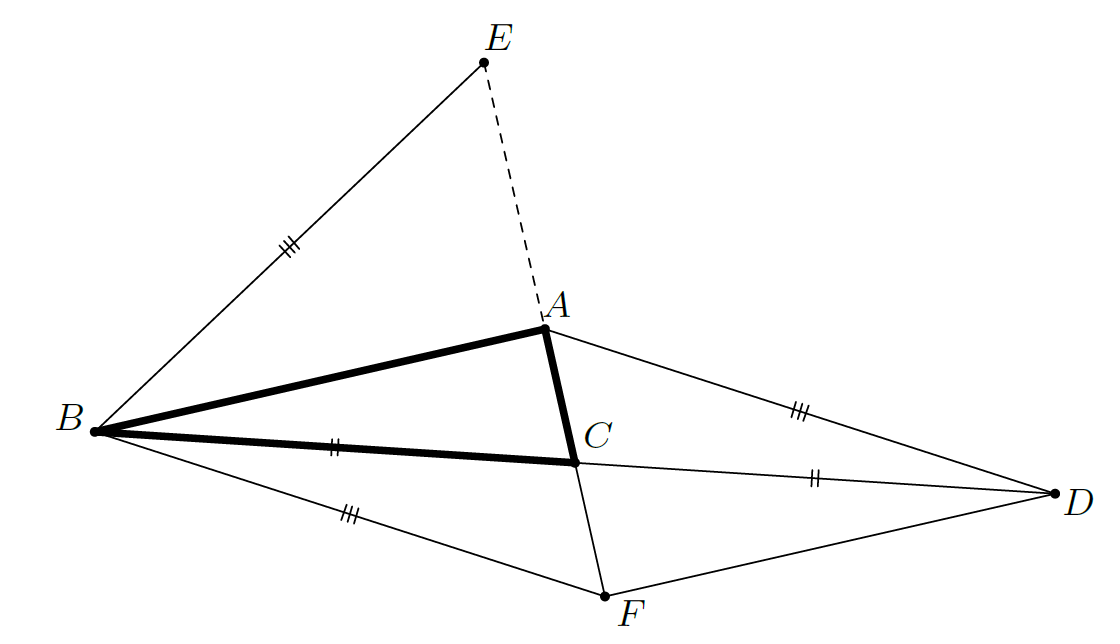
\includegraphics[width=0.4\textwidth]{seniortest1_q1.PNG}
    \end{figure}
    
    % QUESTION 2
    \item[2.] \textit{EGMO 2013, Problem 2} \\
    The solution naturally divides into three different parts: we first obtain some bounds on $m$. We then describe the structure of possible dissections, and finally, we deal with the few remaining cases.
    
    In the first part of the solution, we get rid of the cases with $m \leq 10$ or $m \geq 14$. Let $l_1, \dots, l_5$  and $w_1, \dots, w_5$ be the lengths and widths of the five rectangles. Then the rearrangement inequality yields the lower bound
    \begin{align*}
        l_1 w_1 &+ l_2 w_2 + l_3 w_3 + l_4 w_4 + l_5 w_5 \\
        &= \frac{1}{2} \left( l_1 w_1 + l_2 w_2 + l_3 w_3 + l_4 w_4 + l_5 w_5 + w_1 l_1 + w_2 l_2 + w_3 l_3 + w_4 l_4 + w_5 l_5 \right) \\
        &\geq \frac{1}{2} \left( 1 \cdot 10 + 2 \cdot 9 + 3 \cdot 8 + \dots + 8 \cdot 3 + 9 \cdot 2 + 10 \cdot 1 \right) = 110
    \end{align*}
and the upper bound
    \begin{align*}
        l_1 w_1 &+ l_2 w_2 + l_3 w_3 + l_4 w_4 + l_5 w_5 \\
        &= \frac{1}{2} \left( l_1 w_1 + l_2 w_2 + l_3 w_3 + l_4 w_4 + l_5 w_5 + w_1 l_1 + w_2 l_2 + w_3 l_3 + w_4 l_4 + w_5 l_5 \right) \\
        &\leq \frac{1}{2} \left( 1 \cdot 1 + 2 \cdot 2 + 3 \cdot 3 + \dots + 8 \cdot 8 + 9 \cdot 9 + 10 \cdot 10 \right) = 192.5
    \end{align*}


As the area of the square is sandwiched between $110$ and $192.5$, the only possible candidates for $m$ are $11$, $12$, and $13$.

In the second part of the solution, we show that a dissection of the square into five rectangles must consist of a single inner rectangle and four outer rectangles that each cover one of the four corners of the square. Indeed, if one of the sides the square had three rectangles adjacent to it, removing these three rectangles would leave a polygon with eight vertices, which is clearly not the union of two rectangles. Moreover, since $m > 10$, each side of the square has at least two adjacent rectangles. Hence each side of the square has precisely two adjacent rectangles, and thus the only way of partitioning the square into five rectangles is to have a single inner rectangle and four outer rectangles each covering the four corners of the square, as claimed.

Let us now show that a square of size $12 \times 12$ cannot be dissected in the desired way. Let $R_1, R_2, R_3$ and $R_4$ be the outer rectangles (in clockwise orientation along the boundary of the square). If an outer rectangle has a side of length $s$, then some adjacent outer rectangle must have a side of length $12 − s$. Therefore, neither of $s = 1$ or $s = 6$ can be sidelengths of an outer rectangle, so the inner rectangle must have dimensions $1 \times 6$. One of the outer rectangles (say $R_1$) must have dimensions $10 \times x$, and an adjacent rectangle (say $R_2$) must thus have dimensions $2 \times y$. Rectangle $R_3$ then has dimensions $(12 − y) \times z$, and rectangle $R_4$ has dimensions $(12 - z) \times (12 - x)$. Note that exactly one of the three numbers $x, y, z$ is even (and equals 4 or 8), while the other two numbers are odd. Now, the total area of all five rectangles is
$$ 144 = 6 + 10x + 2y + (12 - y) z + (12 - z)(12 - x), $$

which simplifies to $(y - x)(z - 2) = 6$. As exactly one of the three numbers $x, y, z$ is even, the factors $y - x$ and $z - 2$ are either both even or both odd, so their product cannot equal 6, and thus there is no solution with $m = 12$.

Finally, we handle the cases $m = 11$ and $m = 13$, which indeed are solutions. The corresponding rectangle sets are $10 \times 5, 1 \times 9, 8 \times 2, 7 \times 4$ and $3 \times 6$ for $m = 11$, and $10 \times 5, 9 \times 8, 4 \times 6, 3 \times 7$ and $1 \times 2$ for $m = 13$. These sets can be found by trial and error. The corresponding partitions are shown in the figure below.

    \begin{figure}[h!]
        \centering
        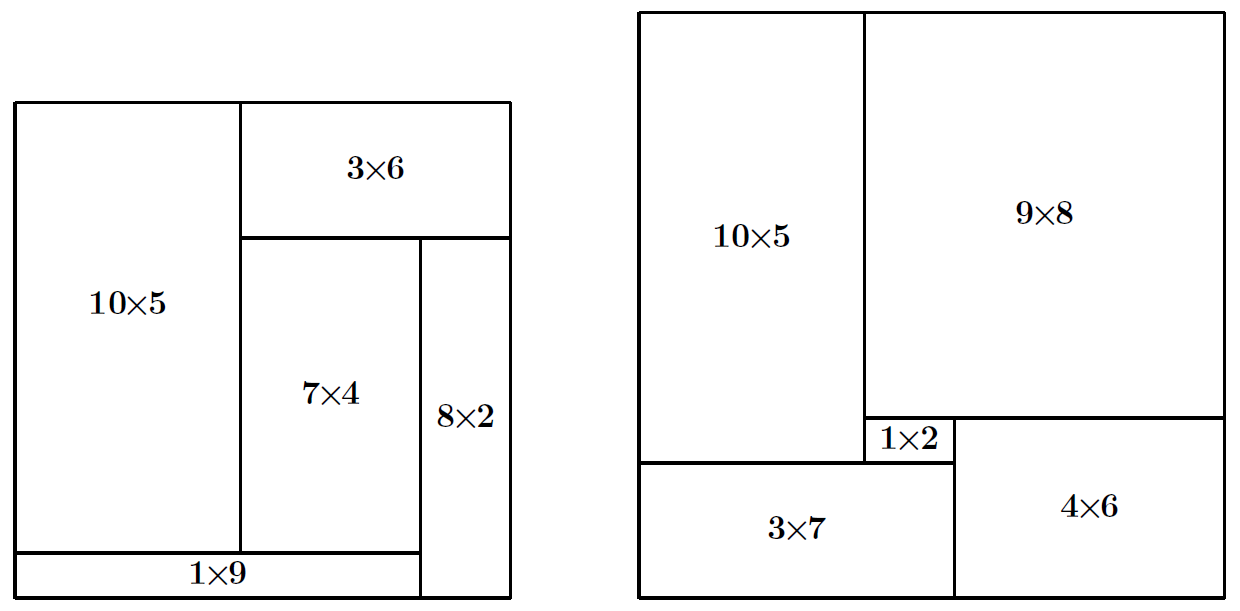
\includegraphics[width=0.8\textwidth]{seniortest1_q2.PNG}
    \end{figure}
    
    \textit{Remark:} The configurations for $m = 11$ and $m = 13$ given above are not unique.

    % QUESTION 3
    \item[3.] We consider two cases: $a \geq 1$ and $a < 1$ . For $a \geq 1$, we have:
    $$ (a^n + 1) \sqrt[n]{a^n + 1} \geq (a^n + 1) a = a^{n+1} + a \geq a^{n+1} + 1 $$
    Taking both sides to the $n$th power gives us the desired inequality for $a \geq 1$. For $a < 1$, noting that $a^n + 1 > a^{n+1} + 1$, we have:
    $$ (a^n + 1)^{n+1} > (a^{n+1} + 1)^{n+1} > (a^{n+1} + 1)^n $$
    which yields the desired inequality.
	
	% QUESTION 4
	\item[4.] \textit{EGMO 2013, Problem 4} \\
	Denote the three consecutive integers by $x - 1$, $x$, and $x + 1$, so that
	\begin{equation} \label{eq1}
	    (x - 1)^5 + a \equiv 0 \quad (\textrm{mod } b), \qquad x^5 + a \equiv 0 \quad (\textrm{mod } b), \qquad (x + 1)^5 + a \equiv 0 \quad (\textrm{mod } b).
	\end{equation}
	
	By computing the differences of the equations in (\ref{eq1}) we get
	\begin{align} \label{eqn2}
	    A &:= (x + 1)^5 - (x-1)^5 = 10x^4 + 20x^2 + 2 \equiv 0 \quad (\textrm{mod } b), \\ \label{eqn3}
	    B &:= (x + 1)^5 - x^5 = 5x^4 + 10x^3 + 10x^2 + 5x + 1 \equiv 0 \quad (\textrm{mod } b).
	\end{align}
	
	Adding the first and third equation in (\ref{eq1}) and subtracting twice the second equation yields
	\begin{equation} \label{eqn4}
	    C := (x + 1)^5 + (x-1)^5 - 2x^5 = 20x^3 + 10x \equiv 0 \quad (\textrm{mod } b).
	\end{equation}
	
	Next, (\ref{eqn2}) and (\ref{eqn4}) together yield
	\begin{equation} \label{eqn5}
	    D := 4xA - (2x^2 + 3)C = -22x \equiv 0 \quad (\textrm{mod } b).
	\end{equation}
	
	Finally we combine (\ref{eqn3}) and (\ref{eqn5}) to derive
	\begin{equation*}
	    22B + (5x^3 + 10x^2 + 10x + 5)D = 22 \equiv 0 \quad (\textrm{mod } b).
	\end{equation*}
	
	As the positive integer $b$ divides $22$, we are left with the four cases $b = 1, b = 2, b = 11$ and $b = 22$.
	
    If $b$ is even (i.e. $b = 2$ or $b = 22$), then we get a contradiction from (\ref{eqn3}), because the integer $B = 2(5x^3 + 5x^2) + 5(x^4 + x) + 1$ is odd, and hence not divisible by any even integer.
    
    For $b = 1$, it is trivial to see that a polynomial of the form $P(n) = n^5 + a$, with $a$ any positive integer, has the desired property.
    
    For $b = 11$, we note that
    \begin{align*}
        n &\equiv 0, 1, 2, 3, 4, 5, 6, 7, 8, 9, 10 \quad (\textrm{mod } 11) \\
        \implies n^5 &\equiv 0, 1, -1, 1, 1, 1, -1, -1, -1, 1, -1 \quad (\textrm{mod } 11)
    \end{align*}
    
    Hence a polynomial of the form $P(n) = (n^5 + a)/11$ has the desired property if and only if $a \equiv \pm 1$ (mod 11). This completes the proof.
	
	% QUESTION 5
	\item[5.] \textbf{Solution 1:} \\
	% Official solution from Croatian 2017, 1.4
	Denote $\alpha = \angle BAC, \beta = \angle CBA$ and $\gamma = \angle ACB$, and let $O$ be the circumcentre of triangle $ABC$.
	
	% DIAGRAM
	
	Point $P$ is on the circle circumscribed to triangle $ACC'$, so $\angle APC = \angle AC'C$ since they are subtended by $\overline{AC}$. Because of the reflection, we have $\angle AC'C = 90^\circ - \angle BAC' = 90^\circ - \alpha$.
	
	Analogously, by observing the circle circumscribed to triangle $ABB'$, we can conclude
	$$ \angle APB = \angle ABB' = 90^\circ - \alpha $$
	Therefore, $\angle CPB = \angle APC + \angle APB = 180^\circ - 2 \alpha$.
	
	Since $AC'PC$ is a cyclic quadrilateral, we have
	$$ \angle CPC' = 180^\circ - \angle CAB - \angle BAC' = 180^\circ - 2 \alpha $$
	
	Therefore, $\angle CPB = \angle CPC'$, so points $P$, $B$, and $C'$ are collinear.
	
	Let $A'$ be the point diametrically opposite point $A$ on the circle circumscribed to triangle $ACC'$. Since $AB$ is the bisector of segment $\overline{CC'}$ point $A'$ lies on line $AB$. Therefore, $\angle A'BP = \angle ABC' = \beta$. By Thales' theorem we have $\angle APA' = 90^\circ$, so
	$$ \angle BPA' = 90^\circ - \angle APB = \alpha $$
	
	Therefore, $\angle AA'P = 180^\circ - \alpha - \beta = \gamma$ and $\angle A'AP = 90^\circ - \angle AA'P = 90^\circ - \gamma$, i.e. $\angle BAP = 90^\circ - \gamma$.
	
	On the other hand, $\angle BOA = 2\gamma$ and $\angle BAO = 90^\circ - \gamma$, so we conclude that $A$, $O$, and $P$ lie on the same line. This completes the proof. \\

% Taariq's solution
\textbf{Solution 2:} \\
    Let $O_1$ and $O_2$ be the centres of circle $CAC^\prime$ and $BAB^\prime$
    respectively. Since $C^\prime$ is the reflection of $C$ about $AB$, we have
    that the perpendicular bisectors of $AC$ and $AC^\prime$ meet on $AB$. It
    follows that $O_1$ lies on $AB$. Similarly, we have that $O_2$ lies on $AC$.
    Now note that $AC$ is the radical axis of the circles $CAC^\prime$ and
    $ABC$, and hence the line $O_1 O$ between their centres is perpendicular to
    $AC$. Thus $O_1 O$ (and similarly, $O_2 O$) is an altitude in the triangle
    $AO_1 O_2$. It follows that $O$ is the orthocentre of $AO_1 O_2$. The line
    $AP$ is the radical axis of circles $CAC^\prime$ and $BAB^\prime$, and hence
    we have that $AP$ is perpendicular to $O_1 O_2$. Thus $AP$ is an altitude of
    $AO_1 O_2$, and hence also passes through the orthocentre $O$.
	
\end{enumerate}
\end{document}





